\documentclass[border=3pt,tikz]{standalone}
\usepackage{amsmath}
\usetikzlibrary{calc}
\usetikzlibrary{arrows.meta} % for arrow size
\begin{document}
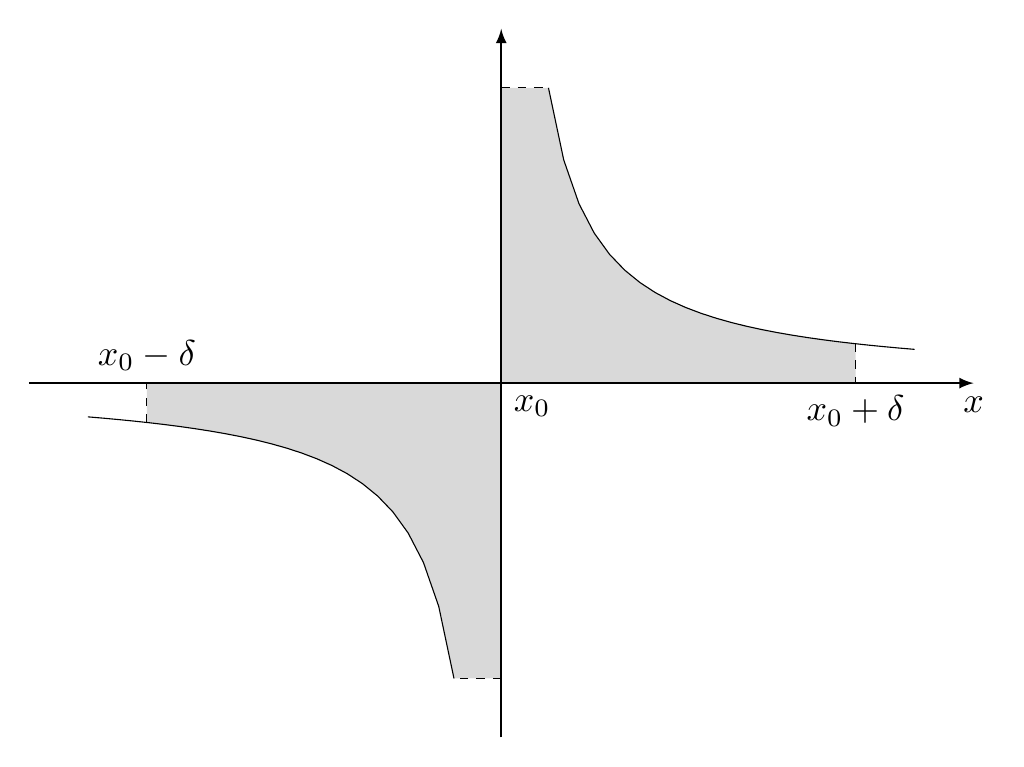
\begin{tikzpicture}[scale=1.5]
    \usetikzlibrary {arrows.meta}
    \usetikzlibrary {calc}  
    \fill [gray!30, domain=0.4:3, variable=\x]
      (0, 2.5)
      -- plot ({\x}, {1/\x})
      -- (3, 0)
      -- (0, 0)
      -- cycle;
    
    \fill [gray!30, domain=-0.4:-3, variable=\x]
      (0, -2.5)
      -- plot ({\x}, {1/\x})
      -- (-3, 0)
      -- (0, 0)
      -- cycle;
    
    \draw [thick, -latex] (-4, 0) -- (4, 0) node[below, scale=1.3] {$x$};
    \draw [thick, -latex] (0, -3) -- (0, 3);
    
    \draw [] plot[domain=-0.4:-3.5, variable=\x] ({\x}, {1/\x});
    \draw [] plot[domain=0.4:3.5, variable=\x] ({\x}, {1/\x});
    \draw[dashed] (0, 2.5) -- (0.4, 2.5);
    \draw[dashed] (3, 0.333) -- (3, 0) node[below, scale=1.3] {$x_0+\delta$};
    
    \draw[dashed] (0, -2.5) -- (-0.4, -2.5);
    \draw[dashed] (-3, -0.333) -- (-3, 0) node[above, scale=1.3] {$x_0-\delta$};
    
    \node[below right, scale=1.3] at (0, 0) {$x_0$};
    \end{tikzpicture}
\end{document}